
\section{Alimentação}


\subsection{Microcontrolador}

Para ambos os microcontroladores testados, STM32 e ESP32,
podem ser usados os pinos de 5v  e 3.3v e a porta micro-USB-B

\subsubsubsection{Pino de 5v não regulado}

Para o ESP32, fontes divergem em relação à tensão mínima e máxima 
que pode ser usada, porém, a maioria concorda em manter de
6v a 7v \cite{esp32_reference_power_supply_1,esp32_reference_power_supply_2, esp32_reference_2}.
Para o STM32 não se encontra informações que discutam o limite máximo de tensão no pino, mas segundo \cite{stm_doc},
o recomendado é manter em 5v.

\subsubsubsection{Pino de 3.3v regulado}
Em ambos as placas, esse pino é mais sensível a variações, pois esta em curto com a alimentação
dos chips, então o ideal é manter entre 3.1v e 3.3v.

\subsubsubsection{Micro-USB-B}
Essa opção permite usar um powerbank, porém o conector das placas é um Micro-USB-B,
modelo que usa protocolo USB 2.0, que pode fornece apenas a 500mA a 5v \cite{micro_usb_b}.
500mA É suficiente para alimentar o ESP32 e o STM32, que podem consumir 
até 260mA \cite{esp_max_current} e 150mA \cite{stm32_datasheet}, respectivamente.

Porem um powerbank pode ser uma solução muito ineficiente do ponto de vista energético,
os modelos populares possuem baterias de lítio de 3.7v, essa tensão é convertido para 5v,
e posteriormente dentro do ESP32 é convertida novamente para 3.3v
No modelo PN-952 da CNHPineng sai de 5000mAh a 3.7v  para 3160mAh a 5v,
podendo novamente perder mais corrente por hora ao ser convertido para 3.3v no ESP32.


\subsection{Motores DC}
Para os motores DC, de 6v, uma bateria de chumbo-ácido de 6v 4,5Ah, 
comumente usada em sistema de câmeras de segurança,
alarmes e iluminação de emergência \cite{bateria_6v_ref_1,bateria_6v_ref_2}.

\begin{figure}[ht]
	\centering
	\caption{Bateria selada de chumbo 6V 4,5Ah}
	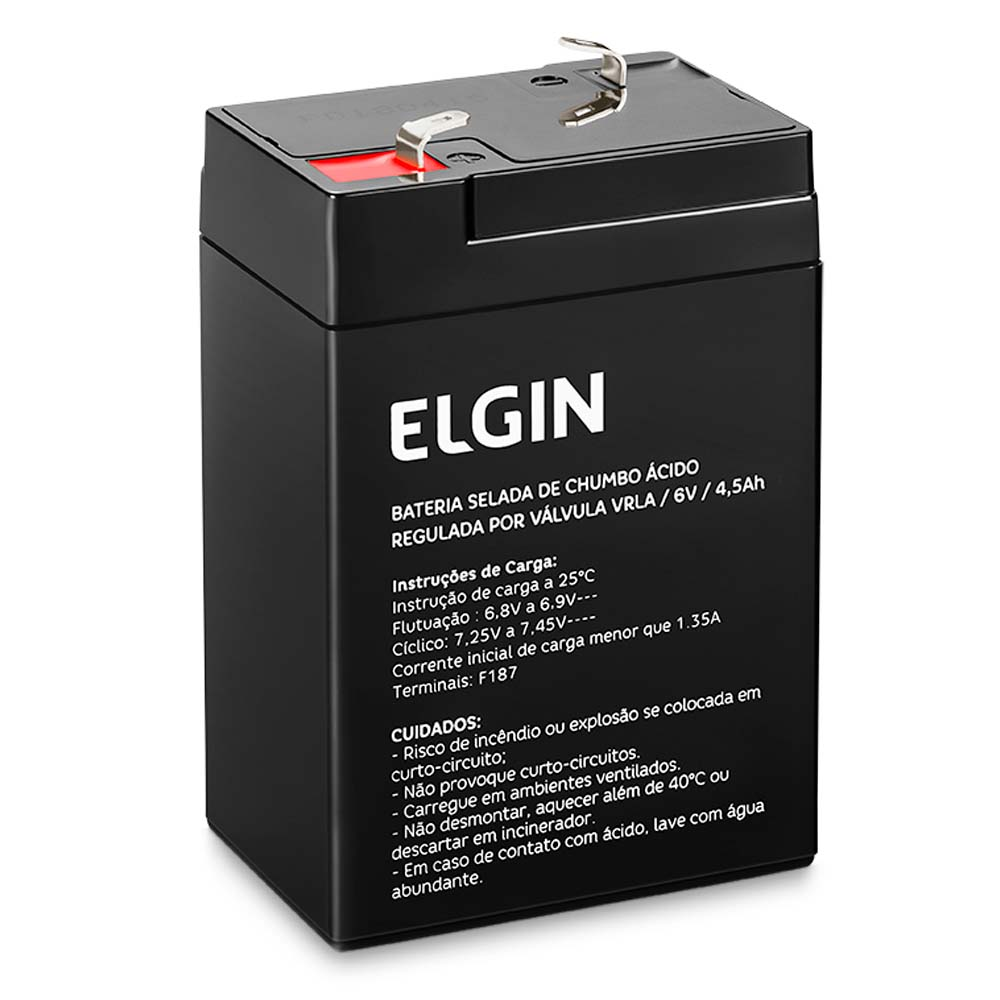
\includegraphics[width=0.4\textwidth]{figures/bateria_6v}
	\fonte{\cite{bateria_6v_ref_1}}
	\label{bateria_6v}
\end{figure}

\subsection{Motores de passo}

Os motores de passo NEMA 17 podem ser alimentados, através do driver, com 12v a 24v.
Observando a possibilidade de uma bateria de 12v/24v ficar sem uso depois do projeto,
e considerando que ferramentas elétricas possuem baterias padronizadas de 12v/18v/36V, 
foi considerando utilizar 3 baterias de 12v da bosch, que já estavam disponíveis para uso.
Cada bateria tem tensão nominal de 12v a 2Ah, do modelo GBA, 
são usadas em aspirador de pó, esmerilhadeiras, furadeiras, plainas e serras circulares.
Conforme as instruções do pacote da bateria tem pico máximo de carga 12v, porém em uso a bateria possui 10.8v,
pois é fabricada com 3 células de 3.6v
Durante os testes com os motores NEMA 17,  as baterias apresentam uma tensão variando de 10.6 a 10.7
Como essas baterias já haviam sido adquiridas antes desse projeto para uso pessoal,
usá-las no projeto se tornou uma opção economicamente viável e sustentável,
já que as baterias ainda usadas em ferramentas pessoais.

\begin{figure}[ht]
	\centering
	\caption{Bateria de ions de litio - Bosch GBA 12v 2Ah}
	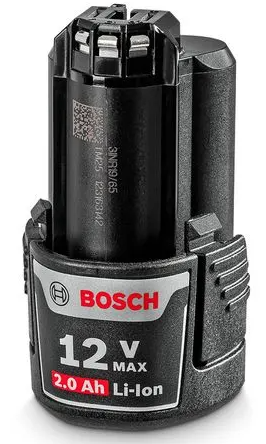
\includegraphics[width=0.25\textwidth]{figures/gba_bosch_bateria}
	\fonte{\cite{bosch_12v}}
	\label{gba_bosch_bateria}
\end{figure}


\begin{figure}[ht]
	\centering
	\caption{Parte de trás da embalagem da bateria Bosch GBA 12v}
	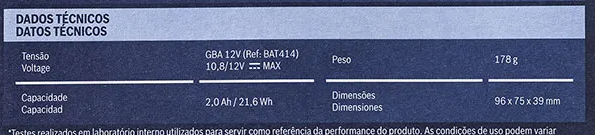
\includegraphics[width=0.8\textwidth]{figures/gba_bosch_embalagem}
	\fonte{\cite{bosch_12v}}
	\label{gba_bosch_embalagem}
\end{figure}

Porém usar essas baterias traz um desafio diferente, a instalação.  Esse tópico é discutido na seção \ref{secao_fabricacao}.

